\documentclass[a4paper, 11pt, oneside]{memoir}

%%%%% Packages %%%%%
\usepackage{lmodern}
\usepackage{palatino}
\usepackage[T1]{fontenc}
\usepackage[utf8]{inputenc}
\usepackage[french]{babel}


%%%%%%%%%%%%%%%%%%%% PACKAGE SECONDAIRE

% \usepackage{amstext,amsmath,amssymb,amsfonts} % package math
% \usepackage{multirow,colortbl}	% to use multirow and ?
% \usepackage{xspace,varioref}
\usepackage[linktoc=all, hidelinks]{hyperref}			% permet d'utiliser les liens hyper textes
\usepackage{float}				% permet d ajouter d autre fonction au floatant
% \usepackage{wrapfig}			% permet d avoir des image avec texte coulant a cote
% \usepackage{fancyhdr}			% permet d inserer des choses en haut et en bas de chaque page
\usepackage{microtype}			% permet d ameliorer l apparence du texte
%\usepackage[explicit]{titlesec}	% permet de modifier les titres
\usepackage{graphicx}			% permet d utiliser les graphiques
\graphicspath{{./images/}}		% to say where are image
% \usepackage{eso-pic} 			% to put figure in the background
\usepackage[svgnames]{xcolor}	% permet d avoir plus de 300 couleur predefini
% \usepackage{array}				% permet d ajouter des option dans les tableaux
% \usepackage{listings}			% permet d ajouter des ligne de code
% \usepackage{tikz}				% to draw figure
% \usepackage{appendix}			% permet de faire les index
% \usepackage{makeidx}			% permet de creer les index
% \usepackage{fancyvrb}			% to use Verbatim
% \usepackage{framed}				% permet de faire des environnement cadre
% \usepackage{fancybox}			% permet de realiser les cadres
%\usepackage{titletoc}			% permet de modifier les titres
\usepackage{caption}
% \usepackage[a4paper, top=2cm, bottom=2cm]{geometry}


\usepackage{graphicx}
\RequirePackage{pageGardeEnsta}	% permet d avoir la page de garde ensta

% \setcounter{secnumdepth}{2}		% permet d'augmenter la numerotation
% \setcounter{tocdepth}{2}		% permet d'augmenter la numerotation

%%%%%%%%%%%%%%%%%% DEFINITION DES BOITES
\newcounter{rem}[chapter]

\newcommand{\remarque}[1]{\stepcounter{rem}\noindent\fcolorbox{OliveDrab}{white}{\parbox{\textwidth}{\textcolor{OliveDrab}{
        \textbf{Remarque~\thechapter.\therem~:}}\\#1}}}

\newcounter{th}[chapter]

\newcommand{\theoreme}[2]{\noindent\fcolorbox{FireBrick}{white}{\stepcounter{th}
    \parbox{\textwidth}{\textbf{\textcolor{FireBrick}{Théorème~\thechapter.\theth~:}}{\hfill \textit{#1}}\\#2}}}

\newcommand{\attention}[1]{\noindent\fcolorbox{white}{white}{\parbox{\textwidth}{\textcolor{FireBrick}{
        \textbf{Attention !}}\\\textit{#1}\\}}}
%%%%%%%%%%%%%%%%%%%%%%%%%%%%%%%%%%%%%%%%%%%%%%%%%%%%%%%%%%%%%%%%%%%%%%%%% 


%% INDEX %%%%%%%%%%%%%%%%%%%%%%%%%%%%%%%%%%%%%%%%%%%%%%%%%%%%
\makeindex

%%%%% Useful macros %%%%%
\newcommand{\latinloc}[1]{\ifx\undefined\lncs\relax\emph{#1}\else\textrm{#1}\fi\xspace}
\newcommand{\etc}{\latinloc{etc}}
\newcommand{\eg}{\latinloc{e.g.}}
\newcommand{\ie}{\latinloc{i.e.}}
\newcommand{\cad}{c'est-à-dire }
\newcommand{\st}{\ensuremath{\text{\xspace s.t.\xspace}}}

%%%% Definition des couleur %%%%

\newcommand\couleurb[1]{\textcolor{SteelBlue}{#1}}
\newcommand\couleurr[1]{\textcolor{DarkRed}{#1}}


%% number page style style %%%%%%%%%%%%%%%%%%%%%%%%%%%%%%%%%%%%%%%%%%%%%%%%%%%%%%

\pagestyle{plain}
% \pagestyle{empty}
% \pagestyle{headings}
% \pagestyle{myheadings}



%% chapters style %%%%%%%%%%%%%%%%%%%%%%%%%%%%%%%%%%%%%%%%%%%%%%%%%%%%%%
%% You may try several styles (see more in the memoir manual).

% \chapterstyle{veelo}
% \chapterstyle{chappell}
% \chapterstyle{ell}
% \chapterstyle{ger}
% \chapterstyle{pedersen}
% \chapterstyle{verville}
\chapterstyle{madsen}
% \chapterstyle{thatcher}


%%%%% Report Title %%%%%
\title{Analyse fonctionnelle}
\author{Équipe Smart}
% \author{\textsc{Rigaud Michaël} \textsc{D'Acremont Antoine} \textsc{Cotten Guillaume} \textsc{Legay Kevin} \textsc{Aya Kenaan} \textsc{Mohamed Shehade}}
\date{\today}
\doctype{Rapport}
\promo{promo 2017}
\etablissement{\textsc{Ensta} Bretagne\\2, rue François Verny\\
  29806 \textsc{Brest} cedex\\\textsc{France}\\Tel +33 (0)2 98 34 88 00\\ \url{www.ensta-bretagne.fr}}
\logoEcole{\includegraphics[height=4.2cm]{logo_ENSTA_Bretagne_Vertical_CMJN}}



%%%%%%%%%%%%%%%%%% DEBUT DU DOCUMENT
\begin{document}

\maketitle
\thispagestyle{empty}
\newpage

\tableofcontents

\newpage
%%%%%%%%%%%%%%%%% INTRODUCTION

\chapter*{Introduction}
\addcontentsline{toc}{chapter}{Introduction}

Ce document constitue le rapport de l'analyse fonctionnelle du projet Smart.
L'équipe Smart est constituée de Rigaud Michaël, D'Acremont Antoine, Cotten Guillaume, Legay Kevin, Aya Kenaan, et Mohamed Shehade.

Le projet Smart a pour but de mettre en place un système de détection et de neutralisation de drones.

Compte tenu du temps imparti, nous avons choisi de nous concentrer sur la détection d'un drone. Pour réaliser cette détection, nous utiliserons un ensemble de goniomètre permettant de réaliser la localisation d'un drone. Ce projet étant nouveau, l'ensemble des recherches et la réalisation du système devront être mené dans le temps imparti.

\newpage

%%%%%%%%%%%%%%%%%%%%%%%% 


\chapter{Recherches}

\section{Présentation du contexte}

Dans le domaine de la détection de drones, après recherche littéraires et numérique, nous en avons conclu qu'il existait plusieurs types de détection: par acoustique, par méthodes optiques et par radiogoniométrie.
Ces méthodes possèdent chacunes leurs avantages et leurs inconvéniants que nous allons spécifier ci-dessous.


\section{Acoustique}

Bonjour
Plusieurs entreprises proposent des outils de détection des drones. Ces derniers se présentent sous forme de boîtiers reliés à des micros, positionnés en hauteur: c'est par le son de leurs hélices que les drones sont repérés, dans un rayon d'une centaine de mètres. Une alerte est alors envoyée sur un ordinateur ou par un SMS. Avantage: le système ne s'occupe pas des ondes, et peut détecter les drones autopilotés (voir plus bas). Problème: le bruit de fond doit être inférieur à un certain seuil, ce qui le rend difficilement utilisable en milieu urbain. De plus, pour des raisons d'échos, la multiplication de récepteurs est nécessaire afin de pouvoir filtrer le signal. Enfin, il est nécessaire de disposer préalablement d'une base de données des signatures acoustiques des différents drones qui peuvent émettre sur un domaine de fréquences acoustiques larges.

Cependant, ce système présente des failles. En effet, il est assez simple pour un drone de parer ce système de détection. Par la simple émission d'une onde sonore couvrant sa propre signature acoustique, un drone passerait totalement inaperçu.

Certains systèmes utilisent aussi une analyse fréquentielle poussée du signal afin de détecter les moteurs en fonction de leurs fréquences de fonctionnement.

Au-delà de cet aspect, il présente un avantage et des plus importants, son coût. En effet, un tel système est très économique à produire. Actuellement diverses solutions actives comme passives sont déjà présentes sur le marché. Ces solutions sont orientées vers une utilisation domestique et non professionnelle pour les raisons évoquées précédemment. Leur prix se situe aux alentours de 100 dollars pour un modèle classique, mais la multiplication des solutions tant à réduire le prix d'un tel système. 

\section{Optique}

Une caméra normale a besoin de lumière pour produire une image, une caméra thermique (ou infrarouge) peut capter de très faibles différences de température et les convertir en une excellente image thermique sur laquelle les plus petits détails sont visibles. Contrairement à d'autres technologies, comme l'amplification de lumière qui nécessite une petite quantité de lumière pour produire une image, l'imagerie thermique permet de voir dans l'obscurité totale. Elle ne nécessite aucune source de lumière.

Depuis qu'il est possible de produire une image lisible dans l'obscurité totale, la technologie de l'imagerie thermique permet de voir et de cibler les forces ennemies dans la nuit la plus noire. Les caméras thermiques voient à travers la brume, la pluie et la neige. Elles voient aussi à travers la fumée, ce qui était particulièrement intéressant pour l'armée.\cite{optique}

En mode passif, \emph{des caméras thermiques d'observation savent repérer un drone de 50 cm d'envergure à une distance d'environ 1 km, de jour comme de nuit} . Lorsqu'un drone entre dans son champ de vision, des algorithmes identifient son image. La forme, la couleur et la géométrie de l'objet permettent de distinguer le drone d'éventuels oiseaux et lancer une alerte, à condition qu'il n'y ait pas d'obstacle entre la caméra et lui.

En mode actif, on peut éclairer une scène à $360^{\circ}$ avec un laser. \emph{Les photons, les particules de lumière, se réfléchissent sur l'appareil, le signal est récupéré et analysé.} D'une portée similaire à celle de la caméra, le laser a l'avantage de \emph{décamoufler} (observation à travers brouillard, pluie ou filet de camouflage), de livrer la distance précise de l'objet, et de le reconstituer en imagerie 3D.Une fois le drone suffisamment proche, une caméra \textit{classique} avec un opérateur humain peuvent prendre le relai pour vérifier visuellement la nature de l'intrus et éventuellement passer à la phase de neutralisation.



\section{Radiogoniométrie}

Parmis les méthodes pour détecter un drone on peut citer la radiogoniométrie. Le principe de la radiogoniométrie est de mesurer la direction d'arrivée d'une onde électromagnétique par rapport à une direction de référence. Les radio-goniomètres sont donc des détecteurs passifs. 

On distingue deux types de goniomètres: les goniomètres à une dimension qui n'estiment que le gisement ou l'azimut, et les goniomètres à deux dimensions qui estiment le gisement ou azimut ainsi que l'élévation. Ainsi grâce à un réseau d'au moins 2 goniomètres il est possible de déterminer la position de l'émission de l'onde.


Dans le cas d'une détection de drones, le radio-goniomètre réalise une écoute de l'environnement avec un balayage de fréquences. Lorsque le drone émettra avec la personne qui le guide on pourra ainsi le localiser précisément.

Seulement, la radiogoniométrie a des failles. En effet, il existe sur le marché des drones auto-pilotés qui n'émettent pas car ils chargent avant le début de leur vol leurs trajectoires. Ainsi il n'y a pas de communication avec un quelconque utilisateur, et donc il n'y a aucun signal émis. Il est donc impossible de les localiser à l'aide de cette technique.

Mais cette technique possède aussi ses avantages. C'est une technique passive et donc indécelable. C'est d'ailleurs pour cela que c'est une technique très utilisée dans la guerre électronique. 





\section{Synthèse}

Ainsi, la meilleure solution serait de réaliser un détecteur à base de ces trois modes de détection. C'est d'ailleurs pourquoi les produits les plus performants existant sur le marché utilisent un mélange de ces trois technologies. On peut notamment citer le cas du système drone-detector \cite{dronedetector}.

Néanmoins nous avons choisi pour ce projet de nous concentrer, dans un premier temps, sur une détection uniquement à base de radiogoniométrie.


%%% Local Variables: 
%%% mode: latex
%%% TeX-master: "rapport_analyse"
%%% End: 

\chapter{Analyse fonctionnel}

Compte tenu des recherches que nous avons réalisées, nous avons établi l'étude fonctionnelle suivante.

\section{Diagramme pieuvre}

\hspace{-2cm}
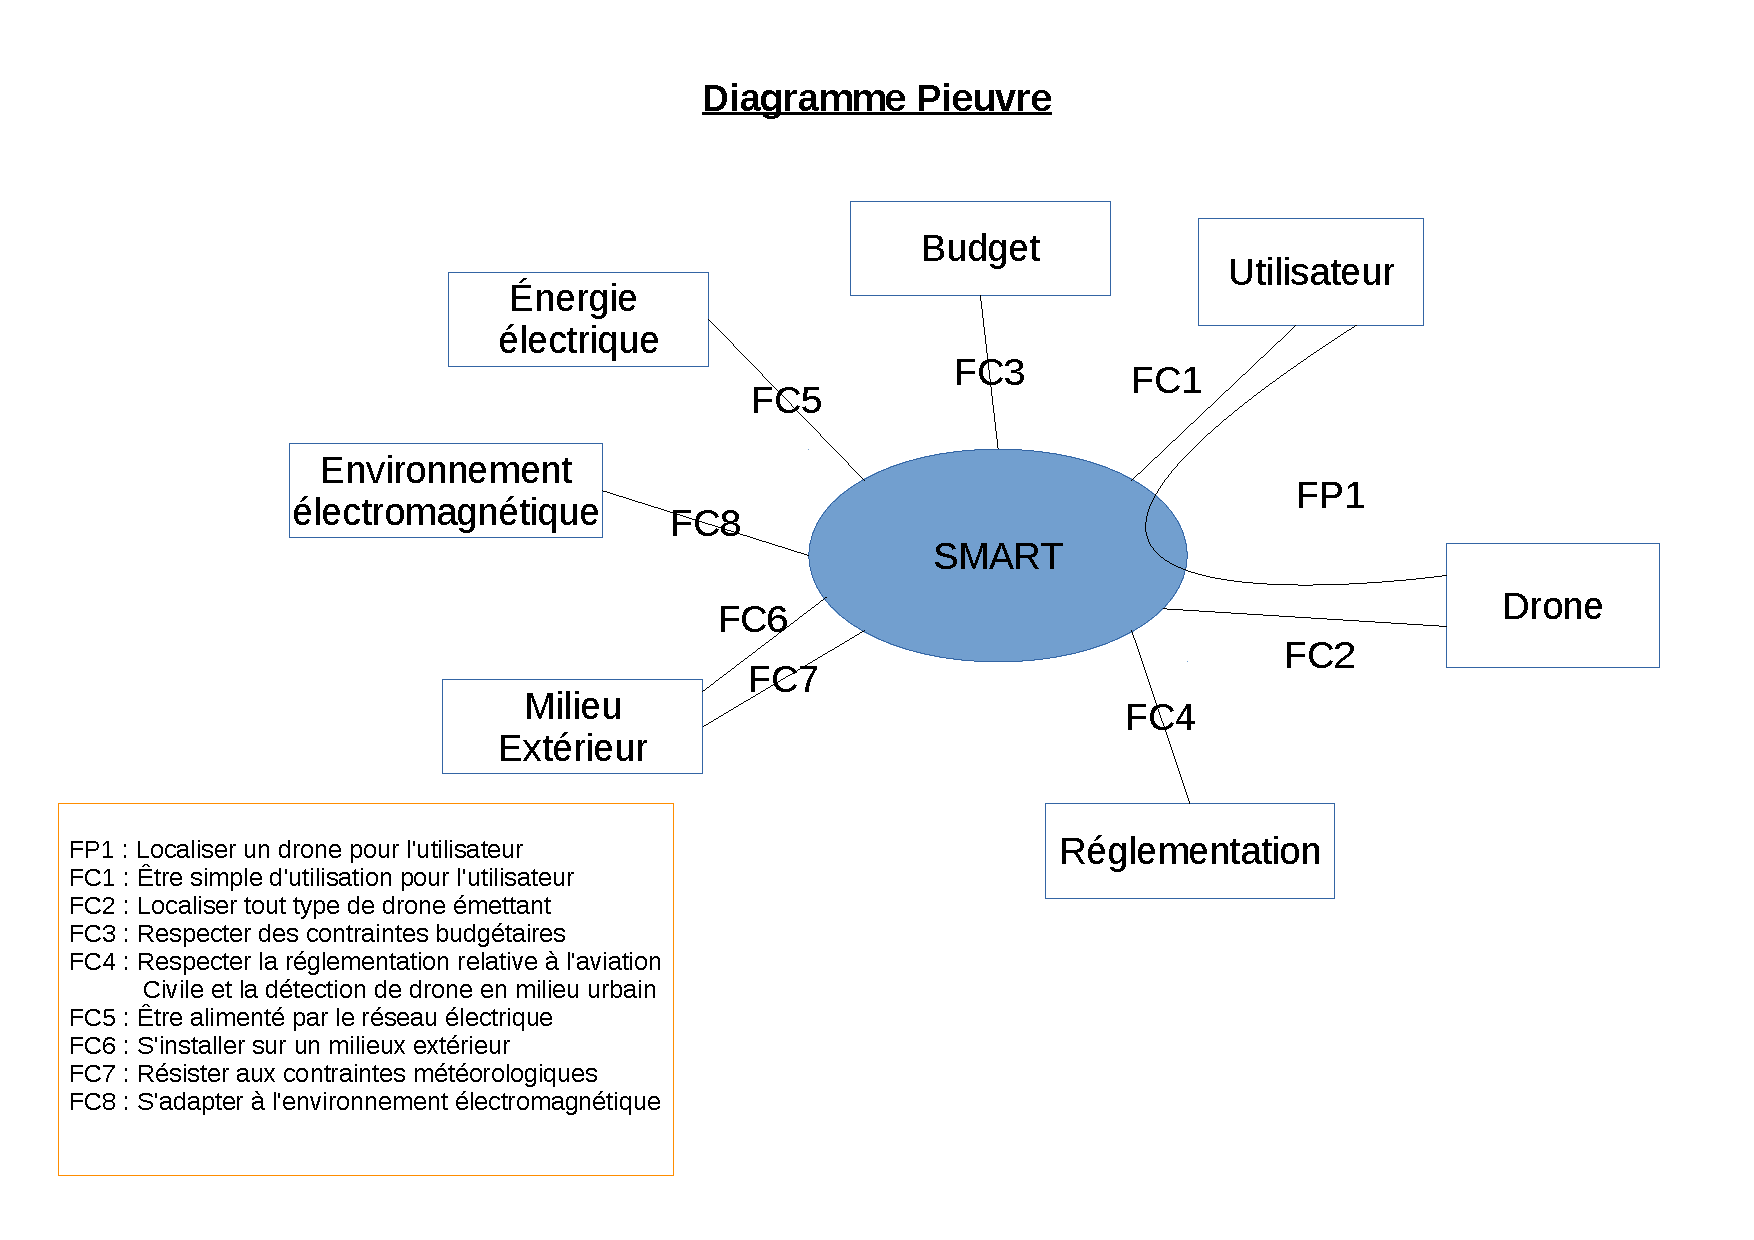
\includegraphics[width=1.18\textwidth]{Diagramme_pieuvre.pdf}
\captionof{figure}{Diagramme pieuvre}



\section{SADT}

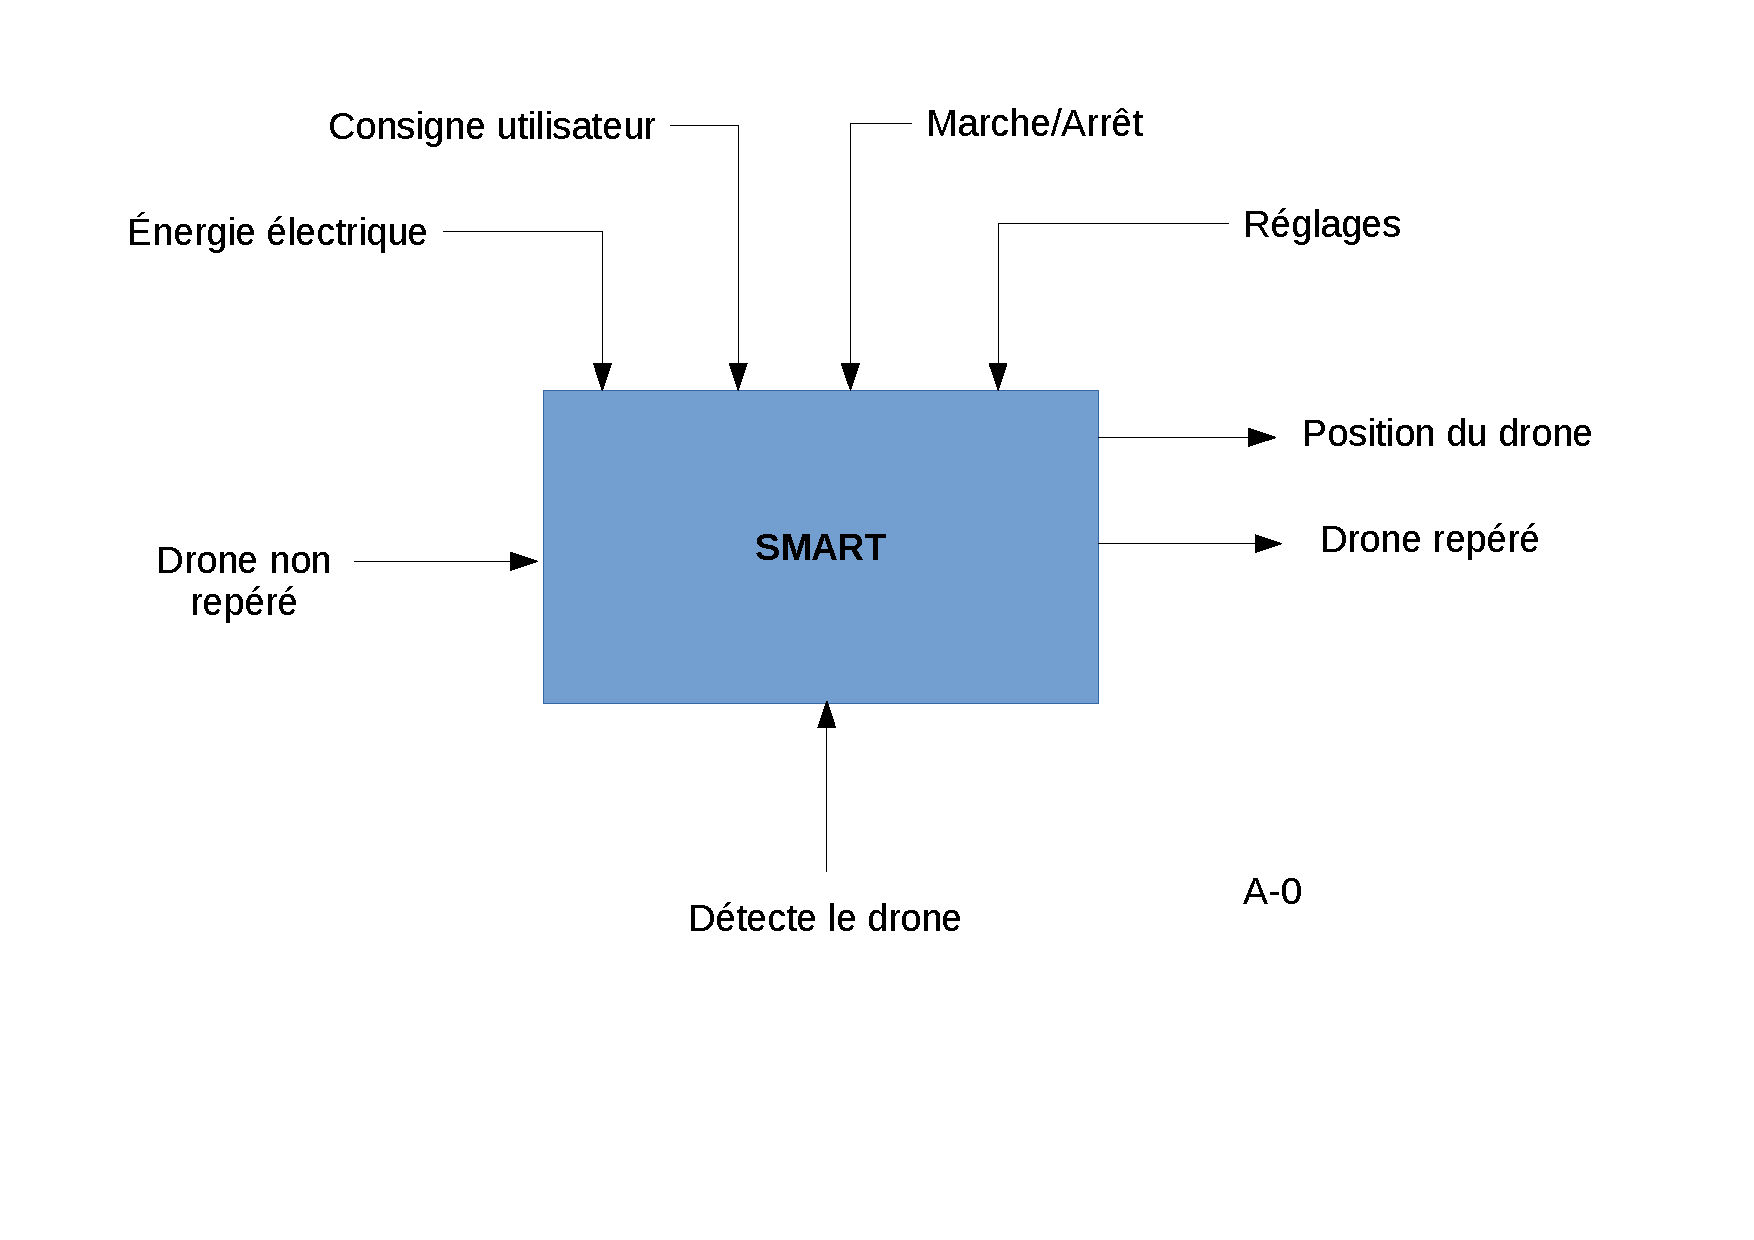
\includegraphics[width=\textwidth]{SADT_A-0.pdf}
\captionof{figure}{SADT A-0}
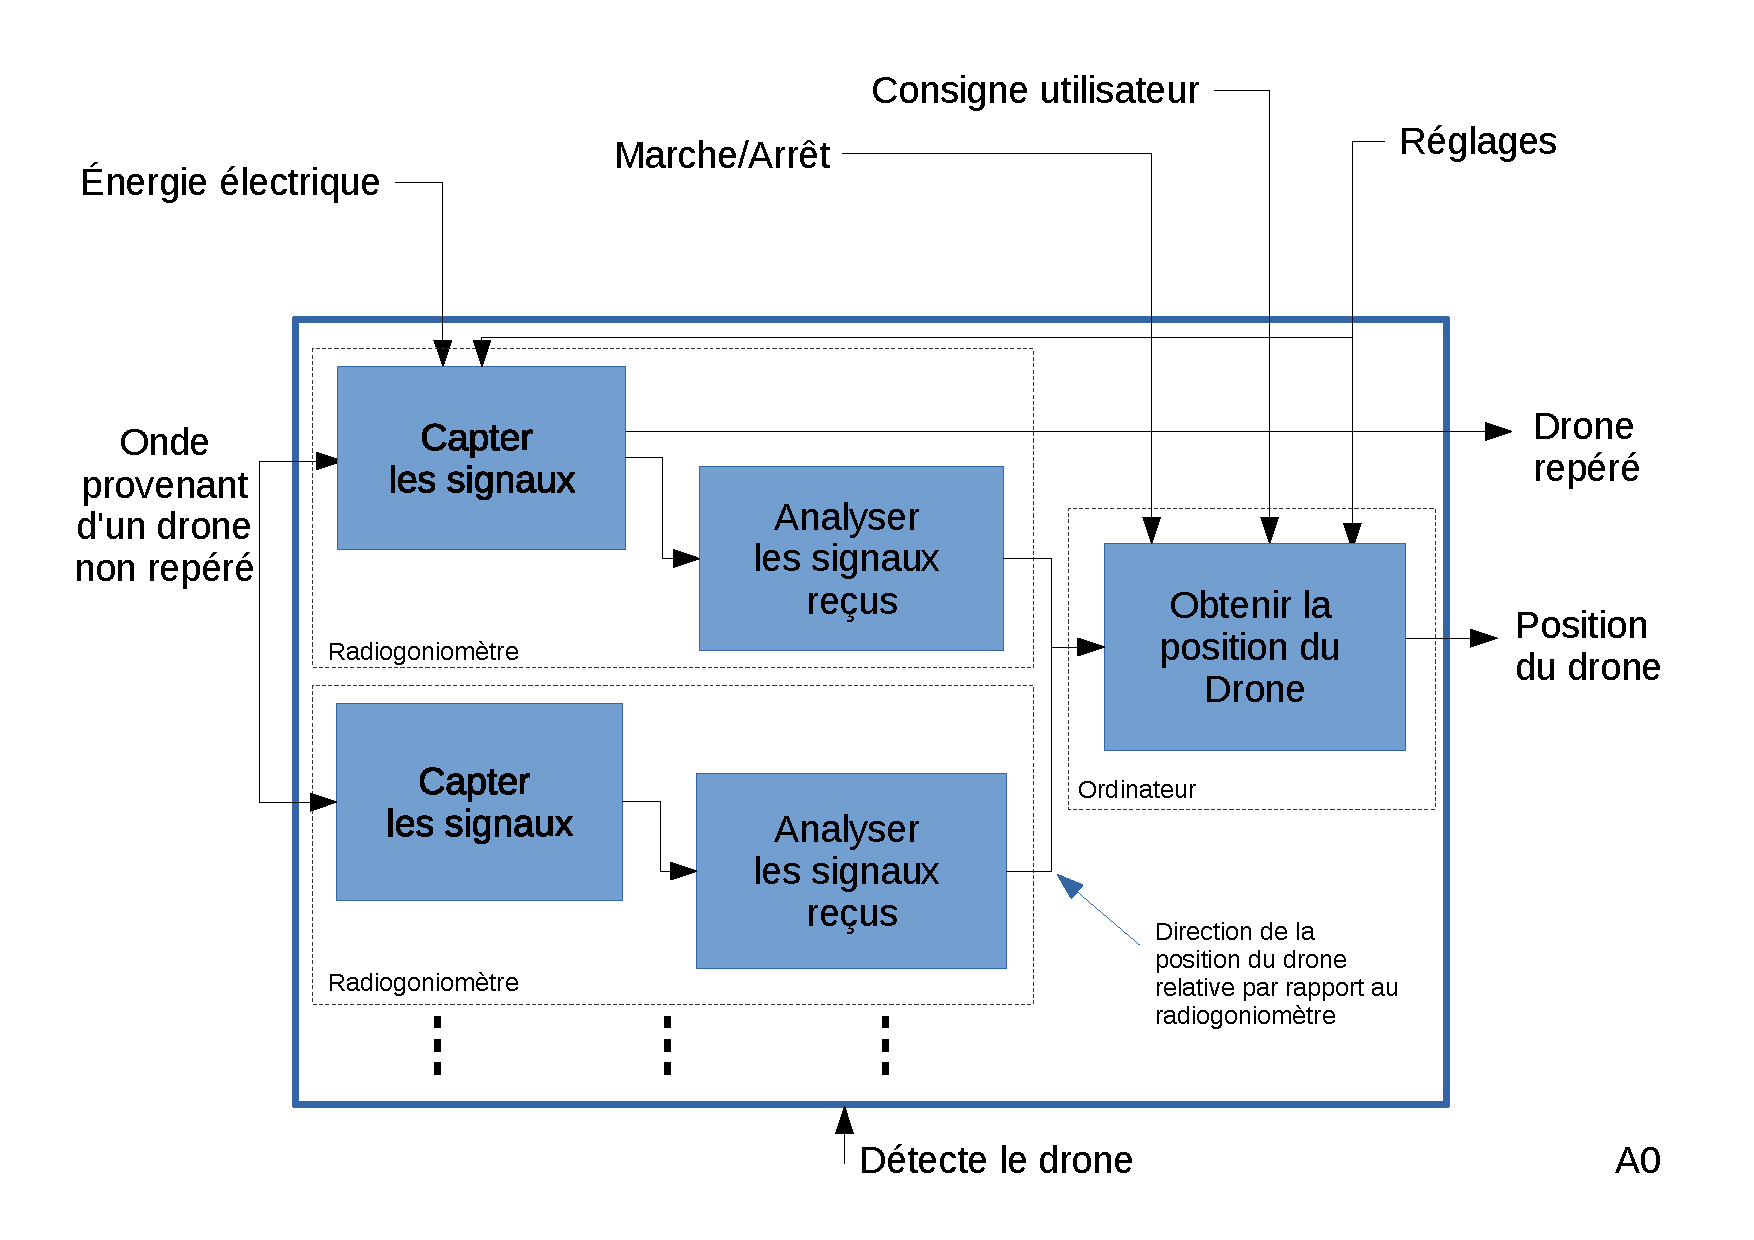
\includegraphics[width=\textwidth]{SADT_A0.pdf}
\captionof{figure}{SADT A0}

\parindent=15pt

Comme on peut le voir sur le SADT A0, nous avons découpé notre objectif en trois parties.

Dans un premier temps il faut capter les signaux. Pour cela il faut réaliser un balayage sur le radiogoniomètre pour détecter les bons signaux.

Ensuite, il faut analyser les signaux reçus pour s'assurer que nous sommes bien en présence d'un drone.

Enfin, il faut récupérer les données des radiogoniometres pour déterminer la position du drone.


\section{Listes des exigences fonctionnelles}

La liste des exigences fonctionnelles est située en Annexe dans le document TableauDesSpecification.xlsx

\section{Cahier des charges}

Le cahier des charges est situé en Annexe dans le document Cahier\_des\_charges.xlsx.




%%% Local Variables: 
%%% mode: latex
%%% TeX-master: "rapport_analyse"
%%% End: 

\chapter{Organisation du travail}


\section{Méthode de travail}

Nous avons cherché au mieux à répartir notre travail. Pour cela nous avons défini 3 grands axes de travail à l'issue de cette étude fonctionnelle.
\begin{itemize}
\item Dans un premier temps nous allons réaliser l'état de l'art.
\item Dans un deuxième temps nous étudierons la phase de réalisation.
\item Enfin nous testerons notre projet dans des conditions réelles.
\end{itemize}
~\\

Tout au long de ce projet nous avons choisi de réaliser notre travail en divisant notre équipe en 3 groupes de travail distincts formés respectivement de D'Acremont - Cotten, Legay - Rigaud, et Kenaan - Shehade. Notamment lors de l'état de l'art, ces groupes vont réaliser des recherches par binômes pour ensuite redistribuer les informations grâce aux outils mis à notre disposition (nous avons détaillé ces outils plus loin).
~\\

De plus, nous avons décidé lors de la phase de conception de diviser ce travail en plusieurs sous ensembles que nous définirons plus tard et qui seront chacun d'eux testés indépendemment, à l'image de tests unitaires en programmation.



\section{Outils utilisés}

Lors de notre projet nous avons choisi d'utiliser plusieurs outils de travail en collaboration.

\begin{itemize}
\item Nous utilisons Office 365. Nous avons créé un groupe de travail où nous partageons des fichiers et envoyons des mails de manière centralisée.
\item Nous utilisons également \LaTeX~pour la rédaction de nos rapports.
\item Nous pensons finalement utiliser Git et GitHub lors de notre phase de conception. Nous avons pour cela crée un projet sur GitHub.
\item Après plusieurs difficultés, nous avons réussi à utiliser Framaboard du groupe Framasoft pour gérer notre projet.
\end{itemize}

~\\
~\\

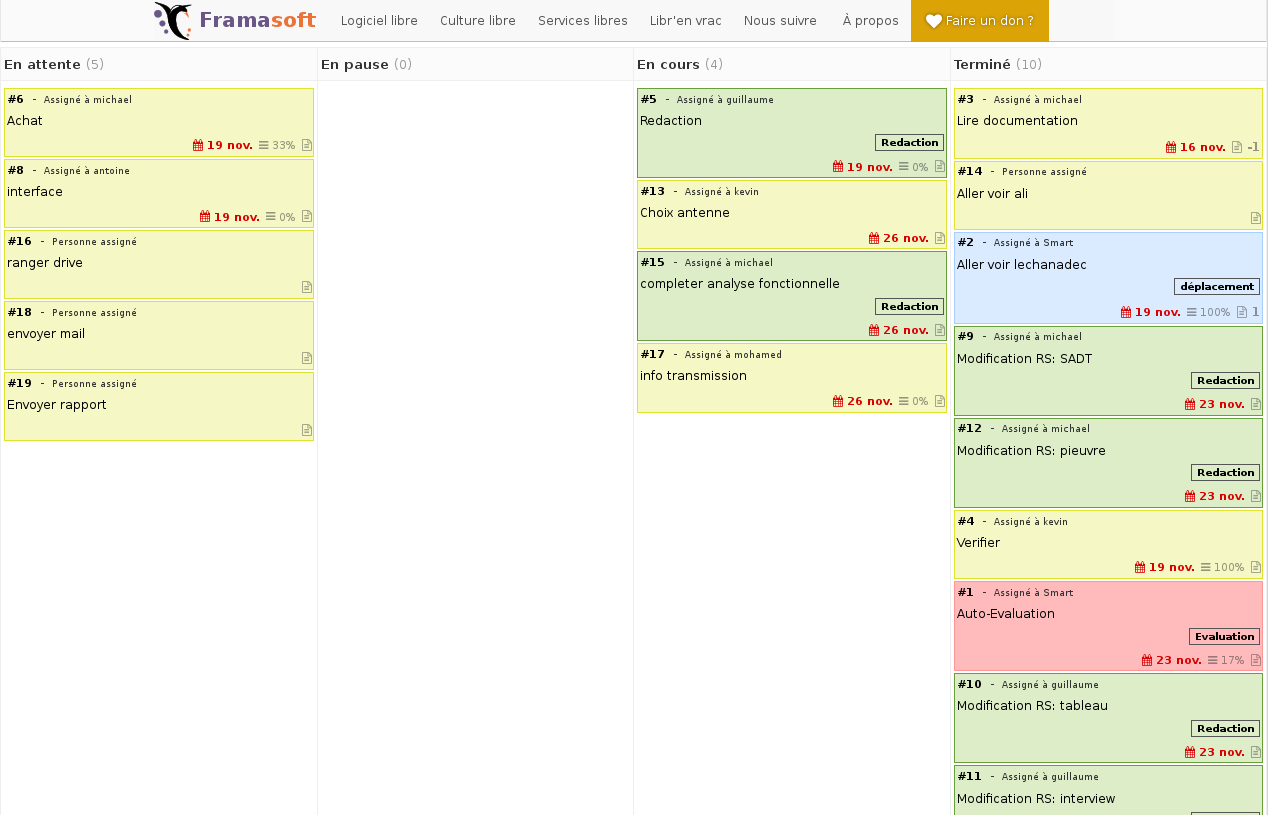
\includegraphics[width=\textwidth]{framaboard}
\captionof{figure}{Impression d'écran de notre Framaboard}
Il est possible d'avoir accès en lecture à notre page Framaboard en cliquant  \textit{\href{https://smart.framaboard.org/?controller=board&action=readonly&token=ab1e20bb26472df067dc24cbd84d9b28eea71bfd68bdea07ab5a9b555ce0}{ici}}






  


%%% Local Variables: 
%%% mode: latex
%%% TeX-master: "rapport_analyse"
%%% End: 



%%%% CONCLUSION %%%%%%%%%

\chapter*{Conclusion}
\addcontentsline{toc}{chapter}{Conclusion}
Bien que sommaire, cette première analyse comprenant de la recherche bibliographique, de la veille technologique et de l'analyse fonctionnelle, nous permet de nous recentrer sur l'essentiel. Le domaine de la localisation de drone étant en plein essor, il est primordial de se concentrer sur un type de détection et d'avancer pas à pas.

Nous allons donc, dès à présent, nous attacher à la compréhension de la radiogoniométrie ainsi qu'à poursuivre la veille technologique afin de retenir les bonnes solutions de détection.

\newpage

%%%% ANNEXE %%%%%%%%%%%%

% \part{Annexe}
\appendix
\nocite{*}
% \input{annexe_}
\newpage
\listoffigures
\printindex
\bibliographystyle{plain}
\bibliography{biblio}

\end{document}
%%%%%%%%%%%%%%%%% FIN DU DOCUMENT
